\documentclass[11pt]{article}
\usepackage[letterpaper,margin=1in]{geometry}
\usepackage[T1]{fontenc}
\usepackage{mathptmx}
\usepackage{amsmath,amssymb}
\usepackage{graphicx}
\usepackage{booktabs}
\usepackage[font=small,labelfont=bf]{caption}
\usepackage[numbers,sort&compress]{natbib}
\usepackage{xcolor}
\usepackage{microtype}
\usepackage{authblk}
\usepackage[colorlinks=true,linkcolor=blue!50!black,citecolor=blue!50!black,urlcolor=blue!50!black]{hyperref}
\setlength{\emergencystretch}{3em}
\renewcommand{\baselinestretch}{1.12}
\newcommand{\LIO}{\texorpdfstring{LaInO$_3$}{LaInO3}}
\newcommand{\BSO}{\texorpdfstring{BaSnO$_3$}{BaSnO3}}
\newcommand{\xmax}{x_\mathrm{max}}
\makeatletter\newcommand{\inputrows}[1]{\@@input #1 }\makeatother

\title{Where the gate charge must sit: electrostatic limits of electrolyte gating at the \LIO/\BSO\ interface and their intersubband signature}
\author{Gracen Ownby}
\affil{University of Oklahoma, Norman, Oklahoma, USA}
\date{\small 13 October 2026}

\begin{document}
\maketitle

\begin{abstract}
Electric-double-layer gating through a 5~nm \LIO\ cap has raised the Hall density of the \LIO/\BSO\ two-dimensional electron gas from about $5\times10^{12}$ to $7.0\times10^{13}$~cm$^{-2}$ at 10~K and $1.08\times10^{14}$~cm$^{-2}$ at 150~K. We ask where the positive charge that balances the added electrons can sit. With a self-consistent Kane-nonparabolic Schr\"odinger--Poisson model of the interface, we place it on the cap surface, as a donor sheet inside the cap, as donors decaying from the surface, or as a uniformly doped layer next to the interface, and require that cap-localized states hold less than 1\% of the electrons. On the cap surface, as an ideal electrolyte double layer, the charge fills the cap by $n_s=2.8$--$3.6\times10^{13}$~cm$^{-2}$; reaching $7\times10^{13}$~cm$^{-2}$ that way would need a conduction-band offset of 3.0--3.5~eV, about twice the measured and calculated 1.35--1.70~eV. The added positive charge must instead lie, on average, within 0.5--1.1~nm of the interface at $7\times10^{13}$~cm$^{-2}$ and within 0.35~nm, less than one \LIO\ unit cell, at $1.08\times10^{14}$~cm$^{-2}$; for a strongly compensated \BSO\ layer the latter density cannot be reached at all. A simple capacitor relation, $\xmax\approx\varepsilon_\mathrm{cap}\varepsilon_0\Delta/(e\,\delta n)$ with $\Delta$ the margin of the field-free cap, reproduces these limits. As a uniform layer of doubly ionized oxygen vacancies next to the interface, the charge corresponds to $\ge1.4\times10^{21}$~cm$^{-3}$ (1.6\% of the oxygen sites) within 0.74~nm. A cap permittivity of 50, twice the measured value, relaxes these distances by factors of 1.9--2.3, and 150~K by at most 0.2~nm; over the literature ranges of the material parameters the distance allowed at $1.08\times10^{14}$~cm$^{-2}$ exceeds one unit cell in 3 of 100 parameter sets. The measured densities are therefore not field effect through the cap but require chemistry at the interface, consistent with the oxygen-vacancy doping suggested by the experimenters. Intersubband absorption cannot tell where the positive charge sits while the cap is empty, because by Gauss's law the \BSO\ side does not depend on it (mean absorption energy within 1.3\%); it does detect cap filling, which holds the \BSO-side density near $3$--$4\times10^{13}$~cm$^{-2}$ and lowers the mean absorption energy by 12--23\% at the same total density.
\end{abstract}

\section{Introduction}
The two-dimensional electron gas (2DEG) at the polar interface between \LIO\ and \BSO\ combines the high room-temperature mobility of \BSO\ with a polarization-induced density of a few $10^{13}$~cm$^{-2}$ \cite{Kim2019LIO,Aggoune2021}. Lee \emph{et al.} raised its density further by electric-double-layer gating with an ionic liquid on a 5~nm \LIO\ cap \cite{Lee2024LIO}: the Hall density rose from about $5\times10^{12}$~cm$^{-2}$ without gate bias to $7.0\times10^{13}$~cm$^{-2}$ at 10~K and $1.08\times10^{14}$~cm$^{-2}$ at 150~K, with a mobility of 2100~cm$^2$/Vs at 10~K, the highest reported for \BSO-based systems. The sheet resistance returned almost to its initial value at zero bias, and the gate leakage stayed below 2~$\mu$A.

Electrolyte gating can act in two ways \cite{Ueno2008,Bisri2017}. In the electrostatic picture the ions form a double layer at the surface, and the gate charge sits a few \aa ngstr\"oms from it. Oxide surfaces can also be reduced: the field drives oxygen out, and the vacancies dope the material electrochemically \cite{Jeong2013,Bisri2017}. For \BSO\ films, gating has been reported to stay reversible over a wide voltage window \cite{Wang2019BSO}. Lee \emph{et al.} noted that oxygen vacancies formed by the ionic liquid near the \LIO\ surface can act as donors in the \LIO\ and help transfer carriers to the interface \cite{Lee2024LIO}.

The cap decides between these pictures. If the added positive charge sits on the cap surface, the field across the cap pulls the cap conduction band down towards the surface; once it reaches the Fermi level, further electrons go into the cap instead of the \BSO\ channel. In a companion study of the intersubband (ISB) optics of this interface we found that this happens after an added density of only $2.0$--$3.1\times10^{13}$~cm$^{-2}$ \cite{OwnbyMAT01}. Here we turn the question around and ask where the positive charge must sit for the interface to reach the measured densities with an empty cap. We map the allowed distance from the interface, the required band offset for an ideal double layer, the allowed share of donors near the surface and the minimum density of a doped layer next to the interface, for compensated and clean \BSO, three cap permittivities, two temperatures and the literature ranges of the \BSO\ parameters. We then ask what ISB absorption can tell: by Gauss's law it is blind to where the positive charge sits as long as the cap is empty, but it detects cap filling.

\section{Model}
\subsection{Interface}
The model is the self-consistent interface solver of Ref.~\cite{OwnbyMAT01}, implemented in qwkit \cite{qwkit}. The conduction band of \BSO\ (band-edge mass $0.19\,m_0$, Kane nonparabolicity $\beta=0.56$~eV$^{-1}$ \cite{Niedermeier2017}, static permittivity 20) and of the \LIO\ cap (offset 1.6~eV \cite{Kim2019LIO,Lee2024LIO,Aggoune2021}, mass $0.46\,m_0$, static permittivity 24 \cite{Jang2017LIO,Galazka2021}, 5~nm thick, closed by a hard wall that stands for the electrolyte) enter a one-band Schr\"odinger equation with energy-dependent mass \cite{Nelson1987}. Each subband has its own in-plane mass and nonparabolicity from the energy-dependent Hamiltonian, Fermi--Dirac occupations, and the Hartree potential follows from Poisson's equation on a 0.5~\AA\ grid. Deep acceptors in the \BSO\ deplete over a width set by Fermi-level pinning 1.0~eV below the bulk conduction band; we consider a strongly compensated layer ($N_A=5\times10^{19}$~cm$^{-3}$, as found in pulsed-laser-deposited films \cite{Kim2019LIO}) and a clean one ($10^{18}$~cm$^{-3}$), closer to the molecular-beam-epitaxy films of Ref.~\cite{Lee2024LIO}. The temperature is 300~K unless stated. Eight subbands enter the self-consistency; at most five are occupied, and the results change by less than $10^{-3}$ in the cap fraction with 14 or 20.

\subsection{Placing the added positive charge}
The interface carries a fixed positive sheet $\sigma_P$ (the compensated polarization charge) chosen so that, with a field-free cap, the ungated density is $n_0=5\times10^{12}$~cm$^{-2}$, the value of Ref.~\cite{Lee2024LIO}. This gives $\sigma_P=4.62\times10^{13}$ and $1.01\times10^{13}$~cm$^{-2}$ for the compensated and clean layers; the difference is the depletion charge. Gating to a density $n_s$ adds $\delta n=n_s-n_0$ electrons, and the same positive charge (plus the small change of the depletion charge) is placed in one of the following ways:
\begin{itemize}
\item at the interface, which leaves the cap field-free (the upper bound on what any placement can reach);
\item as a donor sheet (2~\AA\ wide) a distance $x$ inside the cap; $x=5$~nm is the cap surface, i.e. an ideal electrolyte double layer;
\item as donors decaying from the cap surface with length $\lambda=1$ or 2~nm, with the rest at the interface, a model of vacancies formed at the surface;
\item as a uniformly doped layer of thickness $w$ next to the interface.
\end{itemize}
Donors are taken as fully ionized; the analysis constrains where the ionized (positive) charge is, whatever its origin. Because the system is neutral, the electric field on the \BSO\ side depends only on the electrons and the depletion charge, not on where in the cap the positive charge sits.

\subsection{Criterion}
We call a configuration reachable if cap-localized states (more than half of their weight in the cap) hold less than 1\% of the electrons. The margin $\Delta$ between the lowest cap conduction-band energy and the Fermi level is reported as well; because the lowest cap state lies above the band edge, the 1\% criterion is reached somewhat after $\Delta$ changes sign. For each $n_s$ we find the largest sheet distance $\xmax$, the largest surface share of the donors, the largest layer thickness $w_\mathrm{max}$ and, for the double layer, the smallest offset by bisection.

\subsection{Intersubband observables}
For selected cases the self-consistent potential is extended to all subbands up to 3~eV above the ground subband, and we compute the $k=0$ time-dependent Hartree modes and the $k$-resolved random-phase response of Ref.~\cite{OwnbyMAT01} with the \BSO\ background permittivity including its polar phonons \cite{Stanislavchuk2012}. We report the mean absorption energy $\bar E$ (the oscillator-strength-weighted mean of the mode energies, independent of the linewidth), the median of the absorbed power for a half width of 30~meV, the ISB oscillator strength per electron $f=(2m_0/\hslash^2n_s)\sum_{ab}(n_a-n_b)E_{ba}z_{ab}^2$, whose inverse is the optical mass, and the density held by \BSO-localized subbands, which is what a Hall measurement dominated by the high-mobility channel counts.

\section{Electrostatic limits}\label{sec:limits}
\begin{figure}[t]
\centering
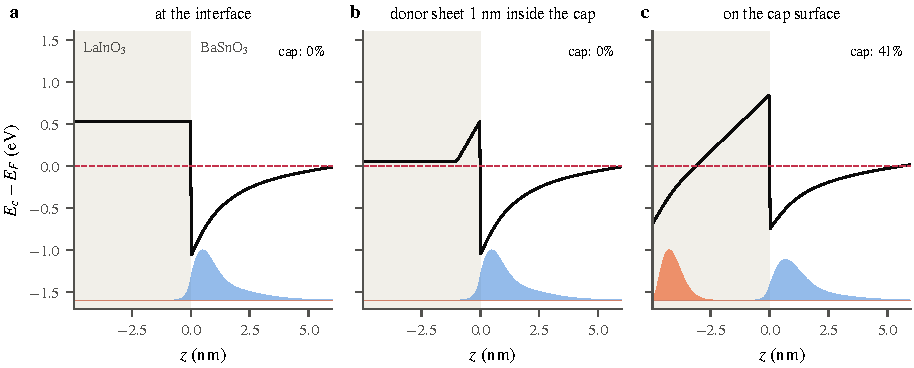
\includegraphics[width=\textwidth]{figures/fig1_profiles.pdf}
\caption{Conduction-band profile (relative to the Fermi level) and electron density in \BSO-localized (blue) and cap-localized (orange) subbands for the clean layer at $n_s=7\times10^{13}$~cm$^{-2}$ ($n_0=5\times10^{12}$~cm$^{-2}$, 300~K), with the added positive charge (a) at the interface, (b) as a donor sheet 1~nm inside the cap and (c) on the cap surface. The cap is shaded.}
\label{fig:prof}
\end{figure}

\subsection{The electrolyte double layer}
Figure~\ref{fig:prof} shows the three basic placements for the clean layer at $7\times10^{13}$~cm$^{-2}$. With the charge at the interface the cap band lies 0.52~eV above the Fermi level; with a donor sheet 1~nm inside the cap the band between the sheet and the surface is lowered to 0.05~eV above it; with the charge on the surface, the cap band falls 0.67~eV below the Fermi level at the surface, and 41\% of the electrons sit in a surface accumulation layer.

The double layer fills the cap early. Cap states hold 1\% of the electrons at $n_s=2.8$ and $3.6\times10^{13}$~cm$^{-2}$ (compensated, clean; Ref.~\cite{OwnbyMAT01}). Raising the offset postpones this, but slowly (Fig.~\ref{fig:lim}b): every $10^{13}$~cm$^{-2}$ of added density needs about 0.44~eV more. At $7\times10^{13}$~cm$^{-2}$ the offset would have to be 3.50 (compensated) or 3.04~eV (clean), and at $1.08\times10^{14}$~cm$^{-2}$ 5.13 or 4.67~eV, against 1.35--1.70~eV from experiment and first-principles calculations \cite{Kim2019LIO,Lee2024LIO,Aggoune2021}. These values exceed the difference of the gaps, 1.0--2.0~eV (\LIO\ 4.1--5.0~eV \cite{Jang2017LIO,Kim2019LIO,Aggoune2021}, \BSO\ about 3.0~eV \cite{Aggoune2022}), so a type-I alignment cannot supply them. A cap permittivity of 50 lowers them by 1.1--1.2~eV at $7\times10^{13}$~cm$^{-2}$ (Table~\ref{tab:map}), still far outside the measured range. The slope follows from the capacitor the cap forms: the field $e\,\delta n/\varepsilon_\mathrm{cap}\varepsilon_0$ across $d=5$~nm drops $e\,\delta n\,d/\varepsilon_\mathrm{cap}\varepsilon_0=0.38$~eV per $10^{13}$~cm$^{-2}$, and the Fermi level rises at the same time.

\begin{figure}[t]
\centering
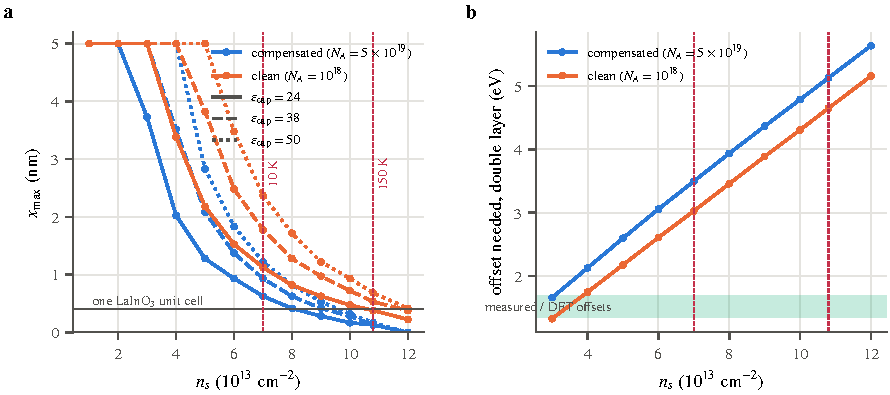
\includegraphics[width=\textwidth]{figures/fig2_limits.pdf}
\caption{(a) Largest distance $\xmax$ of the added positive charge (a donor sheet) from the interface for which cap states hold less than 1\% of the electrons, versus the gated density ($n_0=5\times10^{12}$~cm$^{-2}$, 300~K), for compensated (blue) and clean (orange) \BSO\ and cap permittivities of 24, 38 and 50. The horizontal line marks one \LIO\ pseudocubic cell (0.41~nm); the dashed lines mark the densities measured at 10 and 150~K \cite{Lee2024LIO}. (b) Conduction-band offset needed for the same criterion with all the added charge on the cap surface (cap permittivity 24); the band marks the measured and calculated offsets.}
\label{fig:lim}
\end{figure}

\subsection{How close to the interface}
Figure~\ref{fig:lim}a shows $\xmax$. Up to $3\times10^{13}$~cm$^{-2}$ the charge can sit almost anywhere in the cap. Above that, $\xmax$ falls steeply: at $7\times10^{13}$~cm$^{-2}$ it is 0.47~nm (compensated) and 1.15~nm (clean), and at $1.08\times10^{14}$~cm$^{-2}$ it is 0.35~nm for the clean layer, less than one \LIO\ unit cell. For the compensated layer even charge at the interface does not suffice above $10^{14}$~cm$^{-2}$: with a field-free cap, cap states hold 1.7\% of the electrons at $1.08\times10^{14}$~cm$^{-2}$, because the Fermi level itself reaches the cap band edge.

The limit is a capacitor relation. A sheet at distance $x$ lowers the cap band beyond it by $e\,\delta n\,x/\varepsilon_\mathrm{cap}\varepsilon_0$, so the cap stays empty while this is smaller than the margin $\Delta$ of the field-free cap:
\begin{equation}
\xmax\approx\frac{\varepsilon_\mathrm{cap}\varepsilon_0\,\Delta(n_s)}{e\,\delta n}.\label{eq:xmax}
\end{equation}
For the clean layer this reproduces the computed $\xmax$ to within 0.9~\AA\ from $5\times10^{13}$~cm$^{-2}$ up (for example 10.7 against 11.4~\AA\ at $7\times10^{13}$~cm$^{-2}$); for the compensated layer, whose margin is smaller, it underestimates $\xmax$ by up to 2.3~\AA, because the lowest cap state lies above the band edge. Equation~\eqref{eq:xmax} makes the two ingredients explicit: the margin, which shrinks as the Fermi level rises, and the lever arm, which grows with $\delta n$. Both scale with the cap permittivity only through the second; $\varepsilon_\mathrm{cap}=38$ and 50 raise $\xmax$ by factors of 1.6 and 1.9 for the clean layer at $1.08\times10^{14}$~cm$^{-2}$ (to 0.56 and 0.65~nm).

\begin{table}[t]
\centering\small
\caption{Electrostatic limits at the measured densities ($n_0=5\times10^{12}$~cm$^{-2}$). $\xmax$: largest distance of a donor sheet carrying the added charge; share: largest fraction of the added charge that can sit in donors decaying from the cap surface with length 1~nm (2~nm), the rest at the interface; offset: smallest conduction-band offset for an ideal double layer ($>4$: beyond the search range; the finer scan of Fig.~\ref{fig:lim}b gives 4.67--5.13~eV for permittivity 24). --: not reachable even with the donor sheet next to the interface.}
\label{tab:map}
\begin{tabular}{@{}llcccccc@{}}
\toprule
& & \multicolumn{3}{c}{$n_s=7.0\times10^{13}$~cm$^{-2}$} & \multicolumn{3}{c}{$n_s=1.08\times10^{14}$~cm$^{-2}$} \\
\cmidrule(lr){3-5}\cmidrule(lr){6-8}
\BSO, $T$ & $\varepsilon_\mathrm{cap}$ & $\xmax$ (nm) & share & offset (eV) & $\xmax$ (nm) & share & offset (eV) \\ \midrule
\inputrows{table_map.tex}
\bottomrule
\end{tabular}
\end{table}

\subsection{Distributed donors}
Donors formed at the cap surface and decaying into it are nearly as harmful as the double layer. With a decay length of 1--2~nm and the rest of the added charge at the interface, at most 14--16\% (compensated) or 35--40\% (clean) of it can sit in such donors at $7\times10^{13}$~cm$^{-2}$, and none or 12--13\% at $1.08\times10^{14}$~cm$^{-2}$ (Table~\ref{tab:map}).

A uniformly doped layer next to the interface is the natural form of the charge if the vacancies (or other donors) accumulate there. Its thickness must stay below $w_\mathrm{max}=0.93$~nm (compensated) or 2.25~nm (clean) at $7\times10^{13}$~cm$^{-2}$, so that its donor density must exceed $7.0\times10^{20}$ or $2.9\times10^{20}$~cm$^{-3}$. At $1.08\times10^{14}$~cm$^{-2}$ the clean layer needs $w\le0.74$~nm and at least $1.4\times10^{21}$~cm$^{-3}$; as doubly ionized oxygen vacancies this is 1.6\% of the oxygen sites of \LIO, concentrated in its first two unit cells. At 150~K, the temperature of the highest measured density, $w_\mathrm{max}$ grows to 0.86~nm and the required density falls to $1.2\times10^{21}$~cm$^{-3}$.

\subsection{Temperature, permittivity and material parameters}\label{sec:uq}
Lowering the temperature to 150~K raises $\xmax$ by at most 2~\AA\ and lowers the offsets by at most 0.04~eV at the measured densities (Table~\ref{tab:map}). The cap permittivity matters more, through Eq.~\eqref{eq:xmax}, but even 50, twice the measured value, leaves $\xmax$ at 0.65--0.75~nm for the clean layer at $1.08\times10^{14}$~cm$^{-2}$, and the compensated layer at or below 0.12~nm.

\begin{figure}[t]
\centering
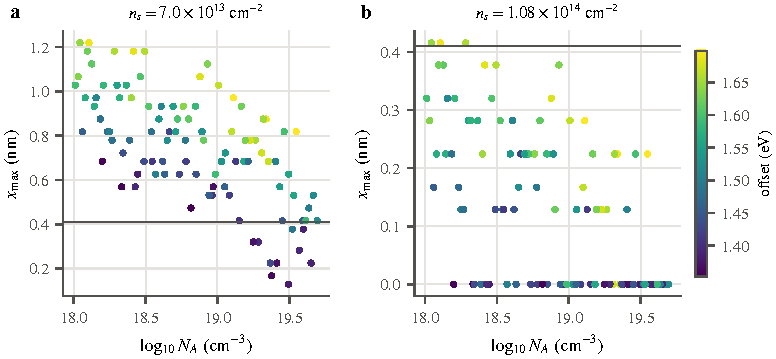
\includegraphics[width=0.85\textwidth]{figures/fig4_uq.pdf}
\caption{Largest distance $\xmax$ of the added positive charge from the interface for the 100 parameter sets of the uncertainty analysis, at the two measured densities ($n_0=5\times10^{12}$~cm$^{-2}$, cap permittivity 24, 300~K), against the acceptor density and colored by the conduction-band offset. $\xmax=0$: cap states hold more than 1\% of the electrons even with the charge next to the interface. The horizontal line marks one \LIO\ unit cell.}
\label{fig:uq}
\end{figure}

The \BSO\ parameters are uncertain as well. We repeated the search for $\xmax$ over the 100 Latin-hypercube parameter sets of the uncertainty analysis of Ref.~\cite{OwnbyMAT01}: band-edge mass 0.17--0.22~$m_0$, nonparabolicity 0.25--0.56~eV$^{-1}$, $\varepsilon_\infty=3.3$--4.3 (with the static permittivity from the Lyddane--Sachs--Teller relation), offset 1.35--1.70~eV, cap mass 0.30--0.50~$m_0$, acceptor density $10^{18}$--$5\times10^{19}$~cm$^{-3}$ (log-uniform) and pinning 0.5--1.5~eV. At $7\times10^{13}$~cm$^{-2}$ the 5th, 50th and 95th percentiles of $\xmax$ are 0.12, 0.73 and 1.13~nm, and in no parameter set may the charge sit even halfway across the cap (Fig.~\ref{fig:uq}a). At $1.08\times10^{14}$~cm$^{-2}$ the field-free cap itself fills in 33 of the 100 sets, the median of $\xmax$ is zero, and $\xmax$ exceeds one unit cell in 3 sets (95th percentile 0.38~nm; Fig.~\ref{fig:uq}b). The rank correlations single out the acceptor density ($-0.72$ and $-0.60$ at the two densities) and the offset ($+0.68$, $+0.59$), followed by $\varepsilon_\infty$ and the mass ($+0.16$ to $+0.29$): less compensation and a larger offset both widen the margin $\Delta$ of Eq.~\eqref{eq:xmax}.

\section{What the intersubband response sees}\label{sec:isb}
\begin{figure}[t]
\centering
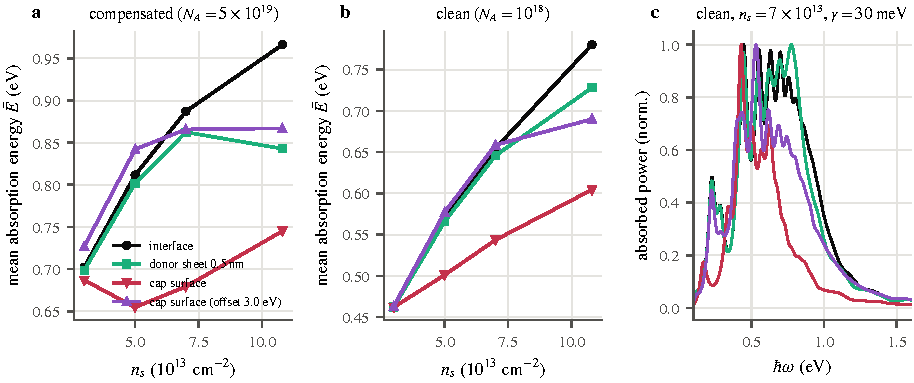
\includegraphics[width=\textwidth]{figures/fig3_isb.pdf}
\caption{(a, b) Mean absorption energy $\bar E$ of the collective ISB response versus the gated density for the four placements of the added positive charge: at the interface, as a donor sheet 0.5~nm inside the cap, on the cap surface, and on the cap surface with a 3.0~eV offset. (c) Absorbed power (half width 30~meV, normalized to its maximum) for the clean layer at $7\times10^{13}$~cm$^{-2}$.}
\label{fig:isb}
\end{figure}

Gauss's law fixes the field on the \BSO\ side by the electrons and the depletion charge alone. As long as the cap is empty, where the positive charge sits in the cap changes only the tails of the subbands in the cap. With a donor sheet 0.5~nm inside the cap instead of at the interface, $E_{21}$ changes by at most 2.4~meV, the mean absorption energy by at most 1.3\% and the median of the absorption by at most 3.1\% wherever the cap holds less than 1\% of the electrons (Fig.~\ref{fig:isb}). A larger offset (3.0~eV, with the charge on the surface) changes $\bar E$ by up to 3.9\%, through the upper subbands that reach into the cap, but leaves the median within 1.4\%. The ISB response therefore cannot distinguish charge at the interface from donors close to it or from a larger offset, and it measures the \BSO-side density whatever the gating mechanism.

It does detect cap filling. With the charge on the cap surface, cap states take up the added electrons: from $5\times10^{13}$~cm$^{-2}$ upwards, the density in \BSO-localized subbands stays at $3.2$--$3.6\times10^{13}$~cm$^{-2}$ (compensated) and $3.9$--$4.4\times10^{13}$~cm$^{-2}$ (clean). At the same total density the mean absorption energy is 12--23\% lower than with the charge at the interface (0.66--0.75 against 0.81--0.95~eV, compensated; 0.50--0.60 against 0.57--0.78~eV, clean), the absorption gains low-energy lines from the cap accumulation layer (Fig.~\ref{fig:isb}c), and the ISB oscillator strength per electron falls from 3.1--3.4 to 2.4--2.9 (compensated) and from 3.5--3.9 to 2.8--3.5 (clean), because the cap electrons are heavier. With the charge at the interface the oscillator strength per electron corresponds to an optical mass of 0.25--0.29~$m_0$ (clean) and 0.29--0.32~$m_0$ (compensated), rising with density through the nonparabolicity.

Two measurements on the same gated sample would thus locate the electrons: the Hall density, which counts the high-mobility \BSO\ channel, and the ISB mean absorption energy, which follows the \BSO-side density along the curve of Fig.~\ref{fig:isb}a,b. If the cap filled, the Hall density would stall near $3$--$4\times10^{13}$~cm$^{-2}$ while the total charge rose, and $\bar E$ would stall with it.

\section{Discussion}\label{sec:disc}
\emph{What the measured densities imply.} The Hall density of Ref.~\cite{Lee2024LIO} counts the high-mobility carriers; a low-mobility channel near the cap surface would add little to it, and the Hall resistance stayed linear up to 7~T. A Hall density of $7\times10^{13}$~cm$^{-2}$ therefore means that many electrons in the \BSO\ channel, and in this model that requires the balancing positive charge within 0.5--1.1~nm of the interface; $1.08\times10^{14}$~cm$^{-2}$ requires it within one \LIO\ unit cell, and a clean \BSO\ layer. Neither is the double layer of an electrostatic gate, which sits 5~nm away. The measured densities therefore point to chemistry at or next to the interface: donors created in the first one or two \LIO\ unit cells, as in the oxygen-vacancy mechanism suggested by the experimenters \cite{Lee2024LIO}, or a change of the interface itself (more polarization charge, or donors on the \BSO\ side). For vacancies formed at the surface to end up there, they must migrate through the cap during gating, which was done at 220~K; that the sheet resistance recovered at zero bias requires the process to be largely reversible.

\emph{Alternatives within the model.} Three parameters could relax the limits. A larger offset helps little: every 0.1~eV raises the margin $\Delta$ by about as much and, by Eq.~\eqref{eq:xmax}, $\xmax$ by only 1.4~\AA\ at $10^{14}$~cm$^{-2}$. A larger cap permittivity helps in proportion (Eq.~\ref{eq:xmax}), but the measured values are 23.7--24.6 \cite{Jang2017LIO,Galazka2021}, and the field between a charge sheet and the interface, $e\,\delta n/\varepsilon_\mathrm{cap}\varepsilon_0\approx7$~MV/cm at $10^{14}$~cm$^{-2}$, would more likely reduce it. Less compensation of the \BSO\ widens the margin most; together with the offset it dominates the uncertainty analysis (Sec.~\ref{sec:uq}), but no parameter set within the literature ranges moves the charge more than a unit cell from the interface at $1.08\times10^{14}$~cm$^{-2}$ in more than 3\% of the cases.

\emph{Limitations.} The envelope-function model is at its limit for confinement within one or two unit cells \cite{OwnbyMAT01}, and the 0.3--0.5~nm distances found at $10^{14}$~cm$^{-2}$ are below the scale on which it describes the interface; they should be read as ``at the interface''. The cap is a continuum with a hard wall, its permittivity is linear, and the donors are point charges smeared over a 2~\AA\ sheet or a uniform layer; exchange and correlation are not included. Defect levels in the cap could hold electrons that do not count as cap subband states; this changes only where the neutral donors sit, not where the ionized charge must be. The Hall density is taken as the \BSO-side density.

\section{Conclusion}
For the \LIO/\BSO\ 2DEG gated through a 5~nm \LIO\ cap, the positive charge that balances the measured electron densities cannot sit in an electrolyte double layer: the cap fills by $2.8$--$3.6\times10^{13}$~cm$^{-2}$, and an offset of 3--5~eV would be needed instead of 1.35--1.70~eV. At $7\times10^{13}$~cm$^{-2}$ the charge must lie within about 1~nm of the interface, at $1.08\times10^{14}$~cm$^{-2}$ within one unit cell, and only for a clean \BSO\ layer; as a doped layer next to the interface this means donor densities of $10^{21}$~cm$^{-3}$, a few percent of the oxygen sites. A capacitor relation captures these limits. Intersubband absorption is insensitive to where the positive charge sits while the cap is empty, which makes it a measure of the \BSO-side density whatever the gating mechanism, and it detects cap filling through a stalled density and a 12--23\% lower mean absorption energy. The calculations use qwkit \cite{qwkit}.

\bibliographystyle{unsrtnat}
\bibliography{refs}
\end{document}
